\chapter{Experimentación y Resultados}\label{chapter:implementation}

En este capítulo se explica cómo se desarrollaron los experimentos realizados, los elementos que formaron 
parte de los mismos, además se se enuncian y justifican algunas de las decisiones tomadas en la implementación
del algoritmo. Por último, se analizan los resultados obtenidos, y si es factible o no la propuesta
para el problema que se quiere resolver.

\section{Detalles de Implementación}
  En la fase de revelación de ofertas se van verificando estas y a la par se van construyendo dos arreglos con las ofertas válidas. Uno de estos arreglos \textit{bidsRevealed} contiene 
  \textit{<value, percent, biderAddress>} (valor, porciento y dirección del postor) de cada oferta. Y
  el otro arreglo \textit{bidsRevealedPercentID} solo contendrá \textit{<percent, id>} (porciento e 
  identificador numérico) de cada oferta válida, cabe destacar que este \textit{id} es la posición del
  arreglo donde se encuentra la oferta, esta información será utilizada más adelante.

  Para determinar los ganadores de la subasta, es necesario seleccionar las mejores ofertas. Para el
  problema actual, que es una variación de la subasta holandesa, las ofertas que ofrecen menores
  porcientos de interés serán las ganadoras. Para escoger estas ofertas, se ordena el arreglo
  \textit{bidsRevealedPercentID}, donde el porciento va a ser el valor por el que se va a hacer el 
  ordenamiento de forma ascendente (de menor a mayor valor). En caso de dos ofertas con igual porciento
  se definirá su orden en dependencia de la que menor \textit{id} tenga.

  Para ordenar el arreglo se hace uso del algoritmo Quick Sort. ¿Por qué se usó Quick Sort y no otro 
  algoritmo de ordenamiento? A pesar de que este algoritmo puede llegar a tener en su peor caso costo
  computacional $O(N^2)$, en el caso promedio se comporta como un algoritmo cuasi lineal $O(N log N)$.
  No se empleó el \textit{merge sort} por la complejidad del lenguaje Solidity en el manejo de la memoria
  y las variables a utilizar, que se deben a las particularidades de la blockchain como nueva tecnología.
  El \textit{merge sort} necesita de un arreglo adicional para ejecutarse y generaría costo 
  computacional adicional, por esta razón no es conveniente su uso. Otra posible opción era el Heap Sort 
  (que no necesita memora adicional), pero 
  se prefirió el empleo del Quick Sort, por la sencillez de su implementación.

  \section{Experimentación}
  \subsection{Tecnologías utilizadas}
    El contrato inteligente que procesa la subasta fue programado en el lenguaje Solidity v0.8.4 
    \parencite{solidity0.8.4}. Para las pruebas realizadas al contrato se utilizó Python 3.8.10 
    \parencite{python3.8} en conjunto con Brownie v1.19.2, este último es un framework basado en Python
    para desarrollar y testear contratos inteligentes dirigidos a ejecutarse en la Máquina Virtual de 
    Ethereum. Además, se empleó Ganache v7.5 \parencite{ganache7.5}, una implementación local de la blockchain de Ethereum, que permite llevar a cabo pruebas de contratos inteligentes sin necesidad de tener una red
    real de Ethereum.

    \subsection{Gas}
      Uno de los conceptos más importantes en el mundo de Ethereum es el Gas. Es una unidad de medida utilizada para medir el trabajo realizado por Ethereum para realizar transacciones o 
      cualquier interacción dentro de la red.


      Una forma sencilla para comprender qué es el Gas en Ethereum sería la siguiente analogía: se quiere viajar 
      de Madrid a Barcelona, el viaje se hará en coche. Se sabe de antemano que son 
      500 km de distancia y que el coche gasta 1 litro de gasolina cada 10 km (para hacer simple el cálculo), 
      así que se necesitará 50 litros de gasolina para llegar al destino. Además, también se sabe que el 
      litro de gasolina cuesta entre 1 € y 1,5 € dependiendo de la gasolinera donde se detenga a repostar.


      Esto es lo mismo que pasa en Ethereum. Por un lado, cada tarea en Ethereum tiene un coste específico 
      y no variable estipulado en Gas, lo que es equivalente al litro de gasolina que gasta el auto por cada 
      10 Km. Por supuesto, las operaciones en Ethereum están formadas por distintas funciones más pequeñas, 
      cada una de ellas con un valor de Gas (o consumo de gasolina) específico y su sumatoria es lo que 
      dirá el valor final en Gas de dicha operación (el total de gasolina a gastar para hacer el viaje).
      Solo resta por responder una interrogante: ¿cuánto se pagará por ese Gas para poder llevar a cabo la operación en Ethereum?

      En la analogía anterior, la gasolina varía entre 1 y 1,5, se puede escoger dónde repostar y pagar lo 
      menos 
      posible para adquirir los 50 litros de gasolina que se necesitan para el viaje. Lo mismo pasa en 
      Ethereum, el Gas tiene un precio en Ether que es dado por la demanda y oferta de operaciones en 
      Ethereum. Es decir, el precio del Gas en Ether es variable, aunque en este caso se puede elegir el 
      valor que se va a pagar por ese Gas, y si un minero está de acuerdo con ese valor, tomará la 
      transacción y la ejecutará.

      Hay tres cosas que son importantes y vitales dentro de Ethereum, y que explicamos a continuación:

      \begin{enumerate}
        \item Unidad de Gas. La Unidad de Gas es la cantidad de Gas que se puede atribuir a una instrucción 
        en específico, pero no tiene ningún valor monetario.
        \item Precio de Gas \textit{gas price}. El Precio de Gas por su parte, es el pago de comisión que se hace por cada Unidad de Gas. Es el precio que se elige pagar por cada unidad y se hace usando unidades decimales de Ether, los llamados Gwei. Esta comisión es la que permite tener prioridad de atención. Si se paga más por cada Unidad de Gas que se use, más rápido los mineros tomarán la transacción y la llevarán a un bloque.
        \item Límite de Gas (\textit{gas limit}). Este es un valor que indica la cantidad máxima de Unidades de Gas que la red 
        Ethereum puede manejar en un momento dado. Es su límite máximo, y un punto que los mineros no 
        pueden sobrepasar en ningún momento.
      \end{enumerate}


      Este último límite es interesante, porque permite hacer frente al problema de la parada 
      (\textit{halting problem}). Este es un 
      problema de computación que permite saber si un programa se ejecutará en un bucle 
      infinito con solo tener a la mano la entrada de datos y su código fuente. Esta situación plantearía un 
      serio problema en la blockchain que podría llevar a una Denegación de Servicios (DoS). Sin embargo, 
      debido a que Ethereum impone un \textit{gas limit} por bloque, esto significa que ninguna operación en 
      Ethereum por compleja que sea podrá exceder jamás dicho límite \parencite{bit2meacademy}. El \textit{gas limit} actual de la red de Ethereum es de 30 Millones \parencite{ycharts}. Figura 
      \ref{figure:smart_contract_squeme}.


      \begin{figure}[h!]
        \centering
        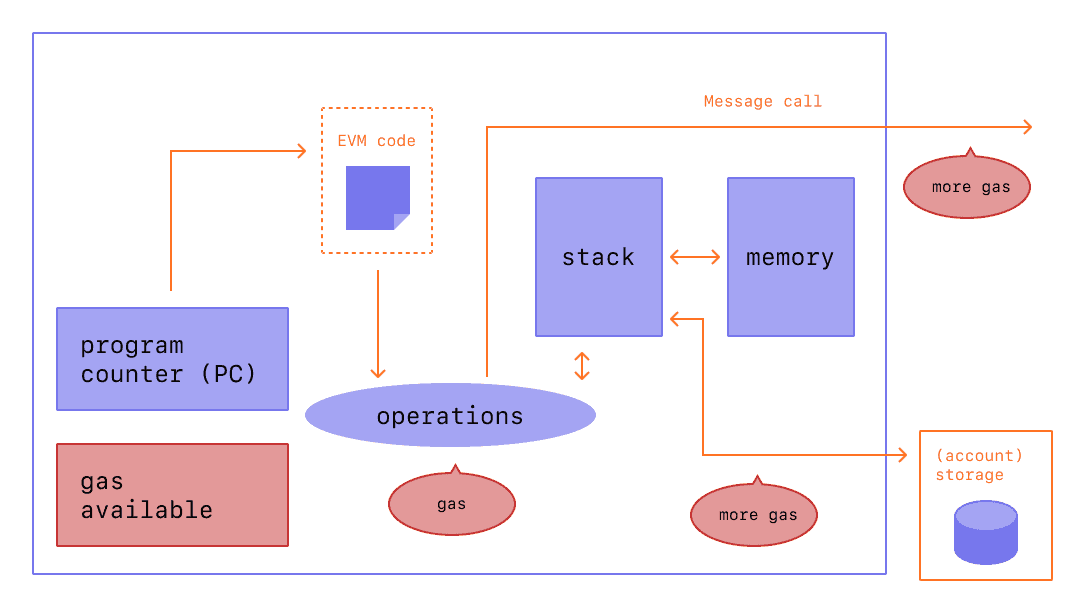
\includegraphics[scale=0.4]{Graphics/gas.png}
        \caption{Diagrama resumen, sobre funcionamiento interno de un contrato inteligente}
        \label{figure:smart_contract_squeme}
      \end{figure}

      \subsubsection{Gas en Quorum}
      Por defecto, la red de Quorum (GoQuorum) es una red libre de gas, lo que significa que el gas no 
      tiene precio (\textit{gas price} igual a 0).


      Las transacciones usan recursos computacionales, por lo que tienen un costo asociado.
      Gas es la unidad de costo y \textit{gas price} es el precio por cada unidad de gas. El costo de
      una transacción es la cantidad de gas empleado multiplicado por el precio del gas. 
      
      En redes públicas como Ethereum, la cuenta que envía la transacción paga el costo de la transacción,
      en Ether. El minero (o validador, en redes con prueba de autoridad) que incluye la 
      transacción en un bloque recibe el costo de la transacción como recompensa.


      En muchas redes privadas, incluyendo GoQuorum, los participantes de la red ejecutan los 
      validadores y no requiere gas como incentivo (como pasa en las redes públicas). Las redes que no 
      requieren gas como incentivo usualmente eliminan el precio del gas o lo configuran para que sea cero
      (gas gratis). Algunas redes privadas pueden distribuir Ether y utilizar un \textit{gas price}
      diferente de cero para limitar el uso de recursos.


      En redes libres de gas, el precio del gas es cero, aunque las transacciones se mantengan usando gas,
      por consiguiente, el costo de la transacción (gas usado por el precio del gas) es cero.


      En GoQuorum, el precio del gas es completamente removido a menos que sea explícitamente habilitado.
      El precio del gas no está incluido entre los parámetros del objeto transacción en los métodos de la
      API privada de GoQuorum \parencite{consensysfreegas}.


      Con lo visto anteriormente se puede concluir que el gas no es totalmente necesario en GoQuorum, ya 
      que no se requiere como incentivo para los mineros, por lo tanto, no se paga por las transacciones
      realizadas en GoQuorum. No obstante, el gas sigue siendo importante para el funcionamiento de
      los contratos inteligentes, por el hecho de que indica la cantidad de recursos computacionales que se requieren para ejecutar una transacción. Y con esto, se puede saber si el algoritmo es eficiente y  escalable. En la siguiente sección se estará abordando este tema.

      \subsection{Pruebas Realizadas}
      Se realizaron varias pruebas al contrato inteligente, para verificar su funcionamiento. En las pruebas 
      iniciales se comprobó que el contrato se desplegara correctamente, y que se pudieran efectuar las 
      transacciones de manera correcta. Luego se hicieron varias pruebas con diferente cantidad de 
      postores y estos a su vez con varias ofertas (válidas e inválidas). La cantidad de postores se 
      escogía de forma aleatoria entre 1 y 12; la cantidad de ofertas de cada postor, también aleatoriamente, entre 1 y 10 ofertas. Finalmente, se efectuaron algunas pruebas de estrés para comprobar los límites máximos de postores y el límite máximo de ofertas válidas.

      En el contrato inteligente, hay 5 métodos que necesitan de transacciones para ejecutarse. Estos son:

      \begin{itemize}
        \item deploy: desplegar el contrato. Esta transacción se lleva a cabo solamente una vez, por el 
        subastador.
        \item bid: enviar una oferta. Esta función puede ser invocada varias veces, por varios postores o por
        el mismo postor. En cada llamado a la función (transacción) se debe enviar un hash (oferta codificada)
        y opcionalmente hacer un depósito en el contrato (no tiene que ser por el mismo valor de la oferta enviada,
        puede ser más o menos que esa cantidad).
        \item reveal: revelar ofertas. Esta función se debe llamar solamente una vez por cada postor. Su
        objetivo es revelar las verdaderas ofertas y clasificarlas en ofertas válidas e inválidas.
        \item auctionEnd: elegir y anunciar ganadores y dar por terminada la subasta. En este método se
        ordenan las subastas válidas, se eligen las mejores hasta completar la totalidad de los bonos
        ofertados.
        \item withdraw: retirar fondos. Cuando se llama a esta función se retiran todos los fondos 
        desbloqueados (depósitos de ofertas inválidas o válidas no ganadoras) pertenecientes a la dirección 
        que envía la transacción.
      \end{itemize}

      En las pruebas realizadas se obtuvo que las funciones usaban la siguiente cantidad de gas para 
      ejecutarse:

      \begin{table}[h!]
        \centering
        \begin{tabular}{|c|c|} \hline
          metodo        & gas usado        \\ \hline
          $deploy$      & $1227782$        \\ \hline
          $bid$         & $[68688, 83700]$ \\ \hline
          $reveal$      & ¿?         \\ \hline
          $auctionEnd$  & ¿?         \\ \hline
          $withdraw$    & $19709$          \\ \hline
        \end{tabular}
        \caption{Gas usado por cada método}
        \label{gas_used}
      \end{table}


      En las funciones \textit{reveal} y \textit{auctionEnd} el gas usado, es variable, depende de las
      condiciones particulares de cada subasta. Tabla \ref{gas_used}.


      \begin{figure}
        \centering
        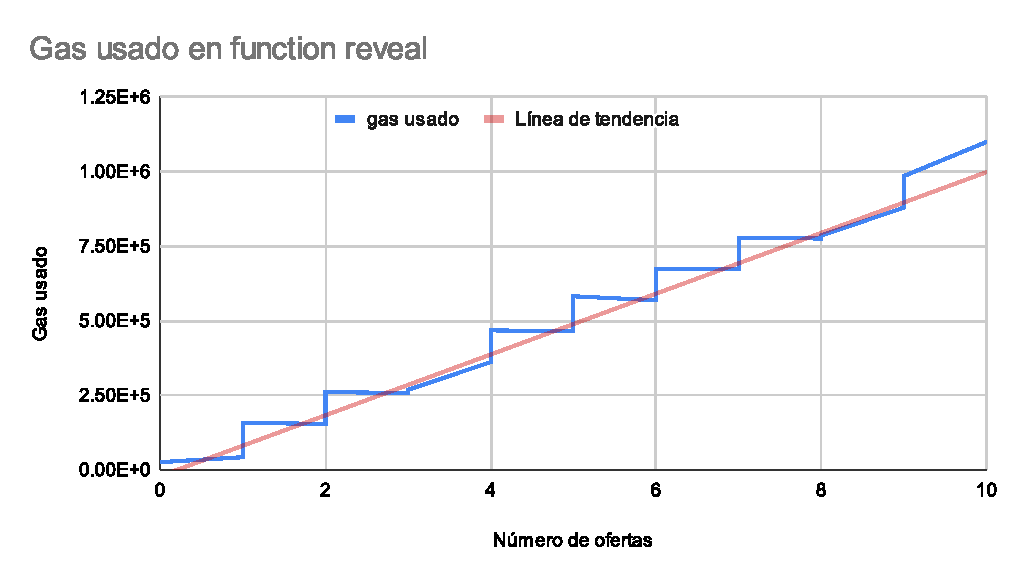
\includegraphics[scale=0.9]{Graphics/gas_reveal.pdf}
        \caption{Gas usado por la función "reveal"}
        \label{gas_reveal}
      \end{figure} 
  
      En la función \textit{reveal} el gas empleado va a depender de la cantidad de ofertas de cada postor.
      Es decir, mientras más ofertas tenga que revelar el postor, mayor será la cantidad de gas que
      consumirá esta. Figura \ref{gas_reveal}.


      \begin{figure}
        \centering
        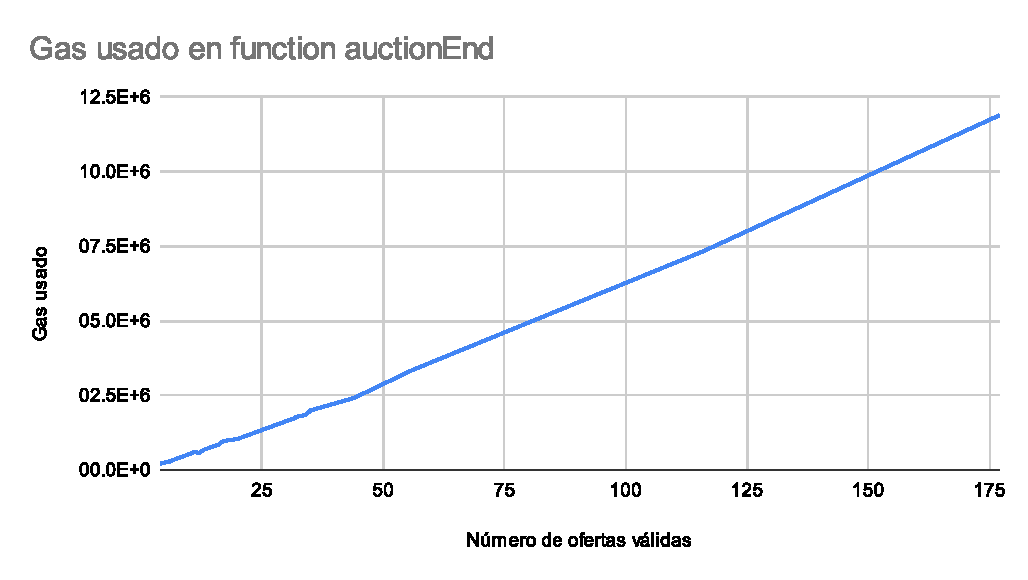
\includegraphics[scale=0.9]{Graphics/gas_auctionEnd.pdf}
        \caption{Gas usado por la función "auctionEnd"}
        \label{gas_auctionEnd}
      \end{figure} 
  
      En la función \textit{auctionEnd} pasa algo similar a la anteriormente vista. El gas empleado va a 
      depender en este caso de la cantidad de ofertas válidas. Es decir, mientras más ofertas válidas tenga 
      la subasta mayor será la cantidad de gas consumido por esta función. Figura \ref{gas_auctionEnd}.


      Para los dos casos anteriores, el gas usado depende cuasi linealmente de la cantidad de ofertas del 
      postor y de la cantidad de ofertas válidas, es decir, si los datos de entrada se duplican, el gas 
      empleado también se duplica.


      En la red local desplegada para probar el contrato inteligente, el límite de gas por bloque es de 
      12 millones (12M) de unidades. Dado este límite y las pruebas de estrés que se le hicieron al 
      algoritmo en esta red local, los límites máximos que las funciones permitían sin exceder el límite
      de gas, y por lo tanto, sin afectar la correcta y completa ejecución del programa, se llegó a los
      siguientes resultados: cantidad máxima de ofertas por un mismo postor fue de 110 aproximadamente,
      y la cantidad de ofertas válidas en la subasta en general de alrededor de 175 ofertas.


      El límite de gas de la red Ethereum actualmente es de 30M \parencite{ycharts}, por lo tanto, en esta red, pudieran ser mayor aún los límites de una subasta realizada con el contrato inteligente propuesto.
      Para predecir los límites en esta red, se usó un algoritmo de regresión lineal, el cual, teniendo 
      los datos de las pruebas en la red local, se obtiene un valor aproximado de cuánto consumiría una 
      ejecución con una cantidad arbitraria de ofertas. Luego de utilizado el algoritmo, el resultado que 
      se obtuvo es que en la red pública de Ethereum se podría efectuar una subasta donde cada postor 
      pusiera a lo más 290 ofertas y que el total de ofertas válidas fuera a lo sumo 440.

  \section{Resultados}
    Teniendo en cuenta los resultados obtenidos en las pruebas realizadas, el algoritmo funciona 
    correctamente y cumple con los objetivos planteados. El contrato inteligente propuesto es factible y 
    útil para ejecutar
    subastas de bonos con ofertas a ciegas en la blockchain de Ethereum o cualquier otra blockchain 
    basada en Ethereum.


    A pesar de que los resultados fueron satisfactorios, también se presentan algunos inconvenientes.
    Las funciones de revelación de ofertas y de fin de subasta, presentan mucho costo computacional para 
    ejecutarse en una blockchain, a medida que aumentan la cantidad de ofertas en la subasta, aumenta 
    proporcionalmente 
    su costo computacional y por consiguiente el gas usado, lo que impide que se ejecute correctamente el contrato
    si se excede el límite de gas de la red utilizada.


    El contrato puede ser empleado, pero a pequeña escala, es necesario que la cantidad de ofertas sea 
    limitada. Por lo tanto, la subasta se debe hacer en un ambiente cerrado, es decir, donde se tenga
    control sobre la cantidad de participantes en la subasta y/o de la cantidad de transacciones realizadas.
    
    No se recomienda ejecutar la subasta en entornos abiertos como Internet, donde muchos tengan acceso al
    contrato, pues de efectuarse un número importante de ofertas en la subasta, el contrato podría tener
    fallos en su funcionamiento y comportamientos inesperados.